\documentclass[twoside]{book}

% Packages required by doxygen
\usepackage{fixltx2e}
\usepackage{calc}
\usepackage{doxygen}
\usepackage{graphicx}
\usepackage[utf8]{inputenc}
\usepackage{makeidx}
\usepackage{multicol}
\usepackage{multirow}
\PassOptionsToPackage{warn}{textcomp}
\usepackage{textcomp}
\usepackage[nointegrals]{wasysym}
\usepackage[table]{xcolor}

% Font selection
\usepackage[T1]{fontenc}
\usepackage{mathptmx}
\usepackage[scaled=.90]{helvet}
\usepackage{courier}
\usepackage{amssymb}
\usepackage{sectsty}
\renewcommand{\familydefault}{\sfdefault}
\allsectionsfont{%
  \fontseries{bc}\selectfont%
  \color{darkgray}%
}
\renewcommand{\DoxyLabelFont}{%
  \fontseries{bc}\selectfont%
  \color{darkgray}%
}
\newcommand{\+}{\discretionary{\mbox{\scriptsize$\hookleftarrow$}}{}{}}

% Page & text layout
\usepackage{geometry}
\geometry{%
  a4paper,%
  top=2.5cm,%
  bottom=2.5cm,%
  left=2.5cm,%
  right=2.5cm%
}
\tolerance=750
\hfuzz=15pt
\hbadness=750
\setlength{\emergencystretch}{15pt}
\setlength{\parindent}{0cm}
\setlength{\parskip}{0.2cm}
\makeatletter
\renewcommand{\paragraph}{%
  \@startsection{paragraph}{4}{0ex}{-1.0ex}{1.0ex}{%
    \normalfont\normalsize\bfseries\SS@parafont%
  }%
}
\renewcommand{\subparagraph}{%
  \@startsection{subparagraph}{5}{0ex}{-1.0ex}{1.0ex}{%
    \normalfont\normalsize\bfseries\SS@subparafont%
  }%
}
\makeatother

% Headers & footers
\usepackage{fancyhdr}
\pagestyle{fancyplain}
\fancyhead[LE]{\fancyplain{}{\bfseries\thepage}}
\fancyhead[CE]{\fancyplain{}{}}
\fancyhead[RE]{\fancyplain{}{\bfseries\leftmark}}
\fancyhead[LO]{\fancyplain{}{\bfseries\rightmark}}
\fancyhead[CO]{\fancyplain{}{}}
\fancyhead[RO]{\fancyplain{}{\bfseries\thepage}}
\fancyfoot[LE]{\fancyplain{}{}}
\fancyfoot[CE]{\fancyplain{}{}}
\fancyfoot[RE]{\fancyplain{}{\bfseries\scriptsize Generated on Thu Dec 11 2014 22\+:42\+:48 for L-\/\+Systems by Doxygen }}
\fancyfoot[LO]{\fancyplain{}{\bfseries\scriptsize Generated on Thu Dec 11 2014 22\+:42\+:48 for L-\/\+Systems by Doxygen }}
\fancyfoot[CO]{\fancyplain{}{}}
\fancyfoot[RO]{\fancyplain{}{}}
\renewcommand{\footrulewidth}{0.4pt}
\renewcommand{\chaptermark}[1]{%
  \markboth{#1}{}%
}
\renewcommand{\sectionmark}[1]{%
  \markright{\thesection\ #1}%
}

% Indices & bibliography
\usepackage{natbib}
\usepackage[titles]{tocloft}
\setcounter{tocdepth}{3}
\setcounter{secnumdepth}{5}
\makeindex

% Hyperlinks (required, but should be loaded last)
\usepackage{ifpdf}
\ifpdf
  \usepackage[pdftex,pagebackref=true]{hyperref}
\else
  \usepackage[ps2pdf,pagebackref=true]{hyperref}
\fi
\hypersetup{%
  colorlinks=true,%
  linkcolor=blue,%
  citecolor=blue,%
  unicode%
}

% Custom commands
\newcommand{\clearemptydoublepage}{%
  \newpage{\pagestyle{empty}\cleardoublepage}%
}


%===== C O N T E N T S =====

\begin{document}

% Titlepage & ToC
\hypersetup{pageanchor=false,
             bookmarks=true,
             bookmarksnumbered=true,
             pdfencoding=unicode
            }
\pagenumbering{roman}
\begin{titlepage}
\vspace*{7cm}
\begin{center}%
{\Large L-\/\+Systems \\[1ex]\large 1.\+0 }\\
\vspace*{1cm}
{\large Generated by Doxygen 1.8.8}\\
\vspace*{0.5cm}
{\small Thu Dec 11 2014 22:42:48}\\
\end{center}
\end{titlepage}
\clearemptydoublepage
\tableofcontents
\clearemptydoublepage
\pagenumbering{arabic}
\hypersetup{pageanchor=true}

%--- Begin generated contents ---
\chapter{Namespace Index}
\section{Namespace List}
Here is a list of all namespaces with brief descriptions\+:\begin{DoxyCompactList}
\item\contentsline{section}{\hyperlink{namespaceoctet}{octet} }{\pageref{namespaceoctet}}{}
\end{DoxyCompactList}

\chapter{Hierarchical Index}
\section{Class Hierarchy}
This inheritance list is sorted roughly, but not completely, alphabetically\+:\begin{DoxyCompactList}
\item app\begin{DoxyCompactList}
\item \contentsline{section}{octet\+:\+:Maths\+\_\+\+L\+\_\+\+Systems}{\pageref{classoctet_1_1_maths___l___systems}}{}
\end{DoxyCompactList}
\item \contentsline{section}{octet\+:\+:L\+\_\+stack}{\pageref{classoctet_1_1_l__stack}}{}
\item \contentsline{section}{octet\+:\+:my\+\_\+vertex}{\pageref{structoctet_1_1my__vertex}}{}
\item \contentsline{section}{octet\+:\+:stk}{\pageref{structoctet_1_1stk}}{}
\end{DoxyCompactList}

\chapter{Class Index}
\section{Class List}
Here are the classes, structs, unions and interfaces with brief descriptions\+:\begin{DoxyCompactList}
\item\contentsline{section}{\hyperlink{classoctet_1_1_l__stack}{octet\+::\+L\+\_\+stack} }{\pageref{classoctet_1_1_l__stack}}{}
\item\contentsline{section}{\hyperlink{classoctet_1_1_maths___l___systems}{octet\+::\+Maths\+\_\+\+L\+\_\+\+Systems} }{\pageref{classoctet_1_1_maths___l___systems}}{}
\item\contentsline{section}{\hyperlink{structoctet_1_1my__vertex}{octet\+::my\+\_\+vertex} }{\pageref{structoctet_1_1my__vertex}}{}
\item\contentsline{section}{\hyperlink{structoctet_1_1stk}{octet\+::stk} }{\pageref{structoctet_1_1stk}}{}
\end{DoxyCompactList}

\chapter{File Index}
\section{File List}
Here is a list of all files with brief descriptions\+:\begin{DoxyCompactList}
\item\contentsline{section}{\hyperlink{main_8cpp}{main.\+cpp} }{\pageref{main_8cpp}}{}
\item\contentsline{section}{\hyperlink{_maths___l___systems_8h}{Maths\+\_\+\+L\+\_\+\+Systems.\+h} }{\pageref{_maths___l___systems_8h}}{}
\end{DoxyCompactList}

\chapter{Namespace Documentation}
\hypertarget{namespaceoctet}{\section{octet Namespace Reference}
\label{namespaceoctet}\index{octet@{octet}}
}
\subsection*{Classes}
\begin{DoxyCompactItemize}
\item 
class \hyperlink{classoctet_1_1_l__stack}{L\+\_\+stack}
\item 
class \hyperlink{classoctet_1_1_maths___l___systems}{Maths\+\_\+\+L\+\_\+\+Systems}
\item 
struct \hyperlink{structoctet_1_1my__vertex}{my\+\_\+vertex}
\item 
struct \hyperlink{structoctet_1_1stk}{stk}
\end{DoxyCompactItemize}

\chapter{Class Documentation}
\hypertarget{classoctet_1_1_l__stack}{\section{octet\+:\+:L\+\_\+stack Class Reference}
\label{classoctet_1_1_l__stack}\index{octet\+::\+L\+\_\+stack@{octet\+::\+L\+\_\+stack}}
}


{\ttfamily \#include $<$Maths\+\_\+\+L\+\_\+\+Systems.\+h$>$}

\subsection*{Public Member Functions}
\begin{DoxyCompactItemize}
\item 
\hyperlink{classoctet_1_1_l__stack_ae51f0abbe777ff635c9222baa23ca49b}{L\+\_\+stack} (float rad, float exelen, mat4t dir)
\item 
void \hyperlink{classoctet_1_1_l__stack_a6ef4bc87ed8db542421d2f8d628d21b7}{push} (uint32\+\_\+t base, float rad, float exelen, mat4t dir)
\item 
void \hyperlink{classoctet_1_1_l__stack_a1d826ecee8e7a32fff42793bedbd1988}{eraseall} ()
\item 
void \hyperlink{classoctet_1_1_l__stack_a7801139caf6842abd54c37c1cd230f1d}{pop} ()
\item 
void \hyperlink{classoctet_1_1_l__stack_ac6ac5ce8c5ed4827eb02cae7a1539a61}{gethead} (uint32\+\_\+t \&base, float \&rad, float \&exelen, mat4t \&dir)
\item 
void \hyperlink{classoctet_1_1_l__stack_a1ff9f3feaeb3d9bf3208cedd16e1ccd5}{sethead} (uint32\+\_\+t base, float rad, float exelen, mat4t dir)
\end{DoxyCompactItemize}
\subsection*{Private Attributes}
\begin{DoxyCompactItemize}
\item 
\hyperlink{structoctet_1_1stk}{stk} $\ast$ \hyperlink{classoctet_1_1_l__stack_aa1205f309b7f112f9145596bf1576a7f}{head}
\end{DoxyCompactItemize}


\subsection{Constructor \& Destructor Documentation}
\hypertarget{classoctet_1_1_l__stack_ae51f0abbe777ff635c9222baa23ca49b}{\index{octet\+::\+L\+\_\+stack@{octet\+::\+L\+\_\+stack}!L\+\_\+stack@{L\+\_\+stack}}
\index{L\+\_\+stack@{L\+\_\+stack}!octet\+::\+L\+\_\+stack@{octet\+::\+L\+\_\+stack}}
\subsubsection[{L\+\_\+stack}]{\setlength{\rightskip}{0pt plus 5cm}octet\+::\+L\+\_\+stack\+::\+L\+\_\+stack (
\begin{DoxyParamCaption}
\item[{float}]{rad, }
\item[{float}]{exelen, }
\item[{mat4t}]{dir}
\end{DoxyParamCaption}
)\hspace{0.3cm}{\ttfamily [inline]}}}\label{classoctet_1_1_l__stack_ae51f0abbe777ff635c9222baa23ca49b}


\subsection{Member Function Documentation}
\hypertarget{classoctet_1_1_l__stack_a1d826ecee8e7a32fff42793bedbd1988}{\index{octet\+::\+L\+\_\+stack@{octet\+::\+L\+\_\+stack}!eraseall@{eraseall}}
\index{eraseall@{eraseall}!octet\+::\+L\+\_\+stack@{octet\+::\+L\+\_\+stack}}
\subsubsection[{eraseall}]{\setlength{\rightskip}{0pt plus 5cm}void octet\+::\+L\+\_\+stack\+::eraseall (
\begin{DoxyParamCaption}
{}
\end{DoxyParamCaption}
)\hspace{0.3cm}{\ttfamily [inline]}}}\label{classoctet_1_1_l__stack_a1d826ecee8e7a32fff42793bedbd1988}
\hypertarget{classoctet_1_1_l__stack_ac6ac5ce8c5ed4827eb02cae7a1539a61}{\index{octet\+::\+L\+\_\+stack@{octet\+::\+L\+\_\+stack}!gethead@{gethead}}
\index{gethead@{gethead}!octet\+::\+L\+\_\+stack@{octet\+::\+L\+\_\+stack}}
\subsubsection[{gethead}]{\setlength{\rightskip}{0pt plus 5cm}void octet\+::\+L\+\_\+stack\+::gethead (
\begin{DoxyParamCaption}
\item[{uint32\+\_\+t \&}]{base, }
\item[{float \&}]{rad, }
\item[{float \&}]{exelen, }
\item[{mat4t \&}]{dir}
\end{DoxyParamCaption}
)\hspace{0.3cm}{\ttfamily [inline]}}}\label{classoctet_1_1_l__stack_ac6ac5ce8c5ed4827eb02cae7a1539a61}
\hypertarget{classoctet_1_1_l__stack_a7801139caf6842abd54c37c1cd230f1d}{\index{octet\+::\+L\+\_\+stack@{octet\+::\+L\+\_\+stack}!pop@{pop}}
\index{pop@{pop}!octet\+::\+L\+\_\+stack@{octet\+::\+L\+\_\+stack}}
\subsubsection[{pop}]{\setlength{\rightskip}{0pt plus 5cm}void octet\+::\+L\+\_\+stack\+::pop (
\begin{DoxyParamCaption}
{}
\end{DoxyParamCaption}
)\hspace{0.3cm}{\ttfamily [inline]}}}\label{classoctet_1_1_l__stack_a7801139caf6842abd54c37c1cd230f1d}
\hypertarget{classoctet_1_1_l__stack_a6ef4bc87ed8db542421d2f8d628d21b7}{\index{octet\+::\+L\+\_\+stack@{octet\+::\+L\+\_\+stack}!push@{push}}
\index{push@{push}!octet\+::\+L\+\_\+stack@{octet\+::\+L\+\_\+stack}}
\subsubsection[{push}]{\setlength{\rightskip}{0pt plus 5cm}void octet\+::\+L\+\_\+stack\+::push (
\begin{DoxyParamCaption}
\item[{uint32\+\_\+t}]{base, }
\item[{float}]{rad, }
\item[{float}]{exelen, }
\item[{mat4t}]{dir}
\end{DoxyParamCaption}
)\hspace{0.3cm}{\ttfamily [inline]}}}\label{classoctet_1_1_l__stack_a6ef4bc87ed8db542421d2f8d628d21b7}
\hypertarget{classoctet_1_1_l__stack_a1ff9f3feaeb3d9bf3208cedd16e1ccd5}{\index{octet\+::\+L\+\_\+stack@{octet\+::\+L\+\_\+stack}!sethead@{sethead}}
\index{sethead@{sethead}!octet\+::\+L\+\_\+stack@{octet\+::\+L\+\_\+stack}}
\subsubsection[{sethead}]{\setlength{\rightskip}{0pt plus 5cm}void octet\+::\+L\+\_\+stack\+::sethead (
\begin{DoxyParamCaption}
\item[{uint32\+\_\+t}]{base, }
\item[{float}]{rad, }
\item[{float}]{exelen, }
\item[{mat4t}]{dir}
\end{DoxyParamCaption}
)\hspace{0.3cm}{\ttfamily [inline]}}}\label{classoctet_1_1_l__stack_a1ff9f3feaeb3d9bf3208cedd16e1ccd5}


\subsection{Member Data Documentation}
\hypertarget{classoctet_1_1_l__stack_aa1205f309b7f112f9145596bf1576a7f}{\index{octet\+::\+L\+\_\+stack@{octet\+::\+L\+\_\+stack}!head@{head}}
\index{head@{head}!octet\+::\+L\+\_\+stack@{octet\+::\+L\+\_\+stack}}
\subsubsection[{head}]{\setlength{\rightskip}{0pt plus 5cm}{\bf stk}$\ast$ octet\+::\+L\+\_\+stack\+::head\hspace{0.3cm}{\ttfamily [private]}}}\label{classoctet_1_1_l__stack_aa1205f309b7f112f9145596bf1576a7f}


The documentation for this class was generated from the following file\+:\begin{DoxyCompactItemize}
\item 
\hyperlink{_maths___l___systems_8h}{Maths\+\_\+\+L\+\_\+\+Systems.\+h}\end{DoxyCompactItemize}

\hypertarget{classoctet_1_1_maths___l___systems}{\section{octet\+:\+:Maths\+\_\+\+L\+\_\+\+Systems Class Reference}
\label{classoctet_1_1_maths___l___systems}\index{octet\+::\+Maths\+\_\+\+L\+\_\+\+Systems@{octet\+::\+Maths\+\_\+\+L\+\_\+\+Systems}}
}


{\ttfamily \#include $<$Maths\+\_\+\+L\+\_\+\+Systems.\+h$>$}

Inheritance diagram for octet\+:\+:Maths\+\_\+\+L\+\_\+\+Systems\+:\begin{figure}[H]
\begin{center}
\leavevmode
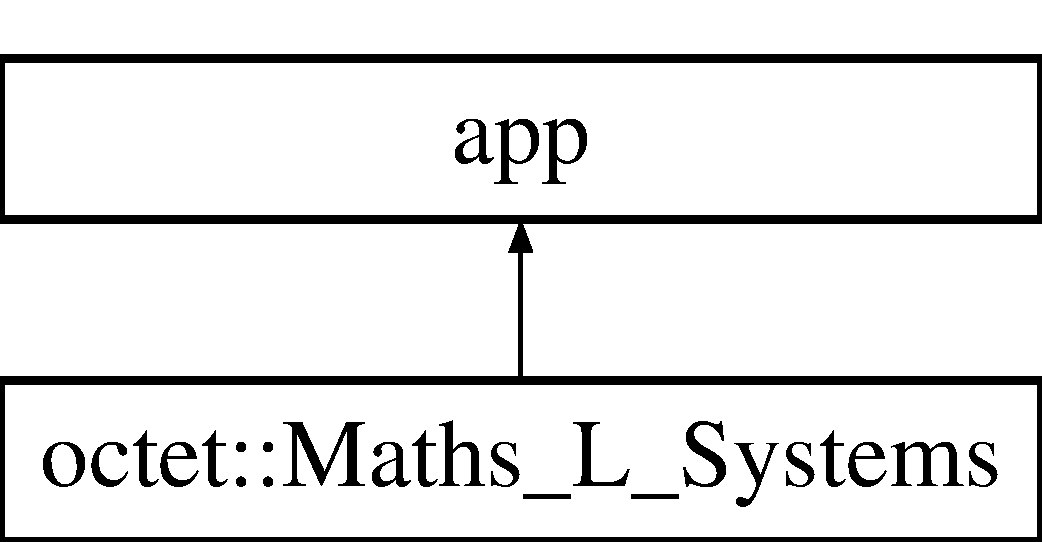
\includegraphics[height=2.000000cm]{classoctet_1_1_maths___l___systems}
\end{center}
\end{figure}
\subsection*{Public Member Functions}
\begin{DoxyCompactItemize}
\item 
\hyperlink{classoctet_1_1_maths___l___systems_aa121ca98ebab9c5c8907c444ae7a770d}{Maths\+\_\+\+L\+\_\+\+Systems} (int argc, char $\ast$$\ast$argv)
\begin{DoxyCompactList}\small\item\em this is called when we construct the class before everything is initialised. \end{DoxyCompactList}\item 
\hyperlink{classoctet_1_1_maths___l___systems_a4ac337cbc5e67002f2bde5b44fa50c14}{$\sim$\+Maths\+\_\+\+L\+\_\+\+Systems} ()
\item 
void \hyperlink{classoctet_1_1_maths___l___systems_a71d9012fc0fbbcd785592af8e129b338}{app\+\_\+init} ()
\begin{DoxyCompactList}\small\item\em this is called once Open\+G\+L is initialized \end{DoxyCompactList}\item 
void \hyperlink{classoctet_1_1_maths___l___systems_a8fa46e98724076f18569e49bcbc7897d}{draw\+\_\+world} (int x, int y, int w, int h)
\begin{DoxyCompactList}\small\item\em this is called to draw the world \end{DoxyCompactList}\end{DoxyCompactItemize}
\subsection*{Private Member Functions}
\begin{DoxyCompactItemize}
\item 
vec3 \hyperlink{classoctet_1_1_maths___l___systems_ad5454ccdf6a5def2e7ff79ea0a729117}{matrixmult} (mat4t objm, vec3 direction)
\begin{DoxyCompactList}\small\item\em This function is used to calu the direction of the camera. \end{DoxyCompactList}\item 
void \hyperlink{classoctet_1_1_maths___l___systems_a738c24b3bbd3bc31d9956eba83bcf90b}{user\+\_\+cont} ()
\begin{DoxyCompactList}\small\item\em The user controls. \end{DoxyCompactList}\item 
int \hyperlink{classoctet_1_1_maths___l___systems_ab9f480dfa7b0201bd097df12d02969ca}{countnumofstep} ()
\begin{DoxyCompactList}\small\item\em This function is used to count the number of variable Symbols in the prarmiter to know the number of verts and indices. \end{DoxyCompactList}\item 
int \hyperlink{classoctet_1_1_maths___l___systems_aa34870a929d313d545957a6845f82a73}{countnumofbranches} ()
\begin{DoxyCompactList}\small\item\em This function is used to count the number of \mbox{[}\mbox{]} in the prarmiter to know the number of verts and indices. \end{DoxyCompactList}\item 
void \hyperlink{classoctet_1_1_maths___l___systems_a3b6f86a6edb2b7728eafb97f6b12a6b9}{interp\+\_\+param} ()
\begin{DoxyCompactList}\small\item\em This function converts the paramiter into the mesh. \end{DoxyCompactList}\item 
void \hyperlink{classoctet_1_1_maths___l___systems_a7e62b7c37a290a739db142859ab15292}{getrule} (int rule\+\_\+number)
\begin{DoxyCompactList}\small\item\em This function is used to fetch the rule from the file. \end{DoxyCompactList}\item 
void \hyperlink{classoctet_1_1_maths___l___systems_aa00aaad8e6c5702c44cc2ffab631c4a8}{iter} (int times)
\begin{DoxyCompactList}\small\item\em This function itirates the current paramiter the number of times indicated and then builds the tree. \end{DoxyCompactList}\item 
void \hyperlink{classoctet_1_1_maths___l___systems_adbd8eaa9e35cc2ff4679bab1be952af9}{create\+\_\+base} ()
\begin{DoxyCompactList}\small\item\em This function creats the base for the scene. \end{DoxyCompactList}\item 
void \hyperlink{classoctet_1_1_maths___l___systems_a8f2e60ebe4f860361a4f99357d4fb240}{Init\+Day\+Night\+Cycle} ()
\begin{DoxyCompactList}\small\item\em This function is used to init the day night cycle. \end{DoxyCompactList}\item 
void \hyperlink{classoctet_1_1_maths___l___systems_adcc1d9dedb89366b1075b72ad79e972b}{Day\+Night\+Cycle} ()
\begin{DoxyCompactList}\small\item\em This function deals with the actual rotation of the dynightcycle node. \end{DoxyCompactList}\end{DoxyCompactItemize}
\subsection*{Private Attributes}
\begin{DoxyCompactItemize}
\item 
ref$<$ visual\+\_\+scene $>$ \hyperlink{classoctet_1_1_maths___l___systems_aca3393864ce7f6347a7d45eac2f21950}{app\+\_\+scene}
\begin{DoxyCompactList}\small\item\em The visual scene. \end{DoxyCompactList}\item 
F\+I\+L\+E $\ast$ \hyperlink{classoctet_1_1_maths___l___systems_a8a58838e93bde57d4d7b1a35cef6e4f2}{L\+\_\+\+Rules}
\begin{DoxyCompactList}\small\item\em The file pointer that we read from. \end{DoxyCompactList}\item 
char $\ast$ \hyperlink{classoctet_1_1_maths___l___systems_a49d998a086a775f7ae692be076e5175d}{current\+\_\+param}
\begin{DoxyCompactList}\small\item\em The L-\/\+System the we are currently making. \end{DoxyCompactList}\item 
int \hyperlink{classoctet_1_1_maths___l___systems_af66610095ffa2515df4b7a821783792d}{number\+\_\+of\+\_\+rules}
\begin{DoxyCompactList}\small\item\em The number of rules this L-\/\+System has. \end{DoxyCompactList}\item 
float \hyperlink{classoctet_1_1_maths___l___systems_a0b97e0018e7e59be5d0e8c268ed85a68}{angle}
\begin{DoxyCompactList}\small\item\em The angle of rotation for the + and -\/ of the L\+\_\+\+System. \end{DoxyCompactList}\item 
float \hyperlink{classoctet_1_1_maths___l___systems_a3baf90aa95cd3c535fba893641f0cd1e}{scale}
\begin{DoxyCompactList}\small\item\em The scaling factor. \end{DoxyCompactList}\item 
char \hyperlink{classoctet_1_1_maths___l___systems_acd98087b379a1b860b1631a6224470e9}{symbols} \mbox{[}5\mbox{]}
\begin{DoxyCompactList}\small\item\em The symbols on the current L-\/\+System. \end{DoxyCompactList}\item 
hash\+\_\+map$<$ char, char $\ast$ $>$ \hyperlink{classoctet_1_1_maths___l___systems_a5c57f1806d42933de86a1d2b2693eb26}{rules}
\begin{DoxyCompactList}\small\item\em The map between the symbols and the rules. \end{DoxyCompactList}\item 
\hyperlink{classoctet_1_1_l__stack}{L\+\_\+stack} $\ast$ \hyperlink{classoctet_1_1_maths___l___systems_a565e71fcec0d1a4d0cca48e99c3b6aca}{var\+\_\+stack}
\begin{DoxyCompactList}\small\item\em The stack variable in which we push and pop the states. \end{DoxyCompactList}\item 
float \hyperlink{classoctet_1_1_maths___l___systems_a3ffafcbe960edcaf6255cc3be7fc10af}{rad}
\begin{DoxyCompactList}\small\item\em The radious of the circle. \end{DoxyCompactList}\item 
float \hyperlink{classoctet_1_1_maths___l___systems_a44da9fdd3c673cac831cf894aa02ec46}{exel}
\begin{DoxyCompactList}\small\item\em The extrution length for the cyln. \end{DoxyCompactList}\item 
scene\+\_\+node $\ast$ \hyperlink{classoctet_1_1_maths___l___systems_ab7bffab6b7ca8de169cccc0dc999a130}{node}
\begin{DoxyCompactList}\small\item\em The node for the mesh. \end{DoxyCompactList}\item 
float \hyperlink{classoctet_1_1_maths___l___systems_acd18538c7b279c111b52f3286be824b3}{initrad}
\begin{DoxyCompactList}\small\item\em The initial radious. \end{DoxyCompactList}\item 
float \hyperlink{classoctet_1_1_maths___l___systems_a0c7beee6e733f6f1912807f2f2912fe8}{initexel}
\begin{DoxyCompactList}\small\item\em The initial extrution length. \end{DoxyCompactList}\item 
int \hyperlink{classoctet_1_1_maths___l___systems_a320a9278ae12e7bed6714027ea64a334}{curr\+\_\+itr}
\begin{DoxyCompactList}\small\item\em The current iteration number. \end{DoxyCompactList}\item 
bool \hyperlink{classoctet_1_1_maths___l___systems_ab9e326a382610ba6088d52a966ec4d9e}{done}
\begin{DoxyCompactList}\small\item\em true if the tree is build \end{DoxyCompactList}\item 
char $\ast$ \hyperlink{classoctet_1_1_maths___l___systems_aec92a84b2e6a408ffe7bdf34ce3285e4}{init\+\_\+param}
\begin{DoxyCompactList}\small\item\em the initial paramiter for the system \end{DoxyCompactList}\item 
bool \hyperlink{classoctet_1_1_maths___l___systems_a656e4a1c5ecad3857ed35fa9b7d27a53}{isday}
\begin{DoxyCompactList}\small\item\em true is its day, false if night \end{DoxyCompactList}\item 
int \hyperlink{classoctet_1_1_maths___l___systems_a1b1840ca480629312bfa309681d6913c}{nightnumber}
\begin{DoxyCompactList}\small\item\em the number of nights that have passed \end{DoxyCompactList}\item 
bool \hyperlink{classoctet_1_1_maths___l___systems_a247062240824f418a425518fdc0d7e58}{enemiesrecycled}
\begin{DoxyCompactList}\small\item\em true if the enemies have been placed in the game , false if not (only used a trigger) \end{DoxyCompactList}\item 
float \hyperlink{classoctet_1_1_maths___l___systems_a6afebf4038c4d8b798e7e35d2b0a9652}{gamedaytime}
\begin{DoxyCompactList}\small\item\em The game day night time (0-\/360) \end{DoxyCompactList}\item 
scene\+\_\+node $\ast$ \hyperlink{classoctet_1_1_maths___l___systems_afdbae311939cba356a0d6fc5c39d1a66}{daynightnode}
\begin{DoxyCompactList}\small\item\em The scene node for the day night cycle objects (sun and moon) \end{DoxyCompactList}\item 
param\+\_\+shader $\ast$ \hyperlink{classoctet_1_1_maths___l___systems_a446a9be9766e7557d06f243a030ab9bf}{shader}
\begin{DoxyCompactList}\small\item\em The shader for the tree. \end{DoxyCompactList}\item 
material $\ast$ \hyperlink{classoctet_1_1_maths___l___systems_aa7cca257e626df634fa52b1a85a1e3d8}{mat\+\_\+tree}
\begin{DoxyCompactList}\small\item\em The material for the tree. \end{DoxyCompactList}\end{DoxyCompactItemize}


\subsection{Constructor \& Destructor Documentation}
\hypertarget{classoctet_1_1_maths___l___systems_aa121ca98ebab9c5c8907c444ae7a770d}{\index{octet\+::\+Maths\+\_\+\+L\+\_\+\+Systems@{octet\+::\+Maths\+\_\+\+L\+\_\+\+Systems}!Maths\+\_\+\+L\+\_\+\+Systems@{Maths\+\_\+\+L\+\_\+\+Systems}}
\index{Maths\+\_\+\+L\+\_\+\+Systems@{Maths\+\_\+\+L\+\_\+\+Systems}!octet\+::\+Maths\+\_\+\+L\+\_\+\+Systems@{octet\+::\+Maths\+\_\+\+L\+\_\+\+Systems}}
\subsubsection[{Maths\+\_\+\+L\+\_\+\+Systems}]{\setlength{\rightskip}{0pt plus 5cm}octet\+::\+Maths\+\_\+\+L\+\_\+\+Systems\+::\+Maths\+\_\+\+L\+\_\+\+Systems (
\begin{DoxyParamCaption}
\item[{int}]{argc, }
\item[{char $\ast$$\ast$}]{argv}
\end{DoxyParamCaption}
)\hspace{0.3cm}{\ttfamily [inline]}}}\label{classoctet_1_1_maths___l___systems_aa121ca98ebab9c5c8907c444ae7a770d}


this is called when we construct the class before everything is initialised. 

\hypertarget{classoctet_1_1_maths___l___systems_a4ac337cbc5e67002f2bde5b44fa50c14}{\index{octet\+::\+Maths\+\_\+\+L\+\_\+\+Systems@{octet\+::\+Maths\+\_\+\+L\+\_\+\+Systems}!````~Maths\+\_\+\+L\+\_\+\+Systems@{$\sim$\+Maths\+\_\+\+L\+\_\+\+Systems}}
\index{````~Maths\+\_\+\+L\+\_\+\+Systems@{$\sim$\+Maths\+\_\+\+L\+\_\+\+Systems}!octet\+::\+Maths\+\_\+\+L\+\_\+\+Systems@{octet\+::\+Maths\+\_\+\+L\+\_\+\+Systems}}
\subsubsection[{$\sim$\+Maths\+\_\+\+L\+\_\+\+Systems}]{\setlength{\rightskip}{0pt plus 5cm}octet\+::\+Maths\+\_\+\+L\+\_\+\+Systems\+::$\sim$\+Maths\+\_\+\+L\+\_\+\+Systems (
\begin{DoxyParamCaption}
{}
\end{DoxyParamCaption}
)\hspace{0.3cm}{\ttfamily [inline]}}}\label{classoctet_1_1_maths___l___systems_a4ac337cbc5e67002f2bde5b44fa50c14}


\subsection{Member Function Documentation}
\hypertarget{classoctet_1_1_maths___l___systems_a71d9012fc0fbbcd785592af8e129b338}{\index{octet\+::\+Maths\+\_\+\+L\+\_\+\+Systems@{octet\+::\+Maths\+\_\+\+L\+\_\+\+Systems}!app\+\_\+init@{app\+\_\+init}}
\index{app\+\_\+init@{app\+\_\+init}!octet\+::\+Maths\+\_\+\+L\+\_\+\+Systems@{octet\+::\+Maths\+\_\+\+L\+\_\+\+Systems}}
\subsubsection[{app\+\_\+init}]{\setlength{\rightskip}{0pt plus 5cm}void octet\+::\+Maths\+\_\+\+L\+\_\+\+Systems\+::app\+\_\+init (
\begin{DoxyParamCaption}
{}
\end{DoxyParamCaption}
)\hspace{0.3cm}{\ttfamily [inline]}}}\label{classoctet_1_1_maths___l___systems_a71d9012fc0fbbcd785592af8e129b338}


this is called once Open\+G\+L is initialized 

\hypertarget{classoctet_1_1_maths___l___systems_aa34870a929d313d545957a6845f82a73}{\index{octet\+::\+Maths\+\_\+\+L\+\_\+\+Systems@{octet\+::\+Maths\+\_\+\+L\+\_\+\+Systems}!countnumofbranches@{countnumofbranches}}
\index{countnumofbranches@{countnumofbranches}!octet\+::\+Maths\+\_\+\+L\+\_\+\+Systems@{octet\+::\+Maths\+\_\+\+L\+\_\+\+Systems}}
\subsubsection[{countnumofbranches}]{\setlength{\rightskip}{0pt plus 5cm}int octet\+::\+Maths\+\_\+\+L\+\_\+\+Systems\+::countnumofbranches (
\begin{DoxyParamCaption}
{}
\end{DoxyParamCaption}
)\hspace{0.3cm}{\ttfamily [inline]}, {\ttfamily [private]}}}\label{classoctet_1_1_maths___l___systems_aa34870a929d313d545957a6845f82a73}


This function is used to count the number of \mbox{[}\mbox{]} in the prarmiter to know the number of verts and indices. 

\hypertarget{classoctet_1_1_maths___l___systems_ab9f480dfa7b0201bd097df12d02969ca}{\index{octet\+::\+Maths\+\_\+\+L\+\_\+\+Systems@{octet\+::\+Maths\+\_\+\+L\+\_\+\+Systems}!countnumofstep@{countnumofstep}}
\index{countnumofstep@{countnumofstep}!octet\+::\+Maths\+\_\+\+L\+\_\+\+Systems@{octet\+::\+Maths\+\_\+\+L\+\_\+\+Systems}}
\subsubsection[{countnumofstep}]{\setlength{\rightskip}{0pt plus 5cm}int octet\+::\+Maths\+\_\+\+L\+\_\+\+Systems\+::countnumofstep (
\begin{DoxyParamCaption}
{}
\end{DoxyParamCaption}
)\hspace{0.3cm}{\ttfamily [inline]}, {\ttfamily [private]}}}\label{classoctet_1_1_maths___l___systems_ab9f480dfa7b0201bd097df12d02969ca}


This function is used to count the number of variable Symbols in the prarmiter to know the number of verts and indices. 

\hypertarget{classoctet_1_1_maths___l___systems_adbd8eaa9e35cc2ff4679bab1be952af9}{\index{octet\+::\+Maths\+\_\+\+L\+\_\+\+Systems@{octet\+::\+Maths\+\_\+\+L\+\_\+\+Systems}!create\+\_\+base@{create\+\_\+base}}
\index{create\+\_\+base@{create\+\_\+base}!octet\+::\+Maths\+\_\+\+L\+\_\+\+Systems@{octet\+::\+Maths\+\_\+\+L\+\_\+\+Systems}}
\subsubsection[{create\+\_\+base}]{\setlength{\rightskip}{0pt plus 5cm}void octet\+::\+Maths\+\_\+\+L\+\_\+\+Systems\+::create\+\_\+base (
\begin{DoxyParamCaption}
{}
\end{DoxyParamCaption}
)\hspace{0.3cm}{\ttfamily [inline]}, {\ttfamily [private]}}}\label{classoctet_1_1_maths___l___systems_adbd8eaa9e35cc2ff4679bab1be952af9}


This function creats the base for the scene. 

\hypertarget{classoctet_1_1_maths___l___systems_adcc1d9dedb89366b1075b72ad79e972b}{\index{octet\+::\+Maths\+\_\+\+L\+\_\+\+Systems@{octet\+::\+Maths\+\_\+\+L\+\_\+\+Systems}!Day\+Night\+Cycle@{Day\+Night\+Cycle}}
\index{Day\+Night\+Cycle@{Day\+Night\+Cycle}!octet\+::\+Maths\+\_\+\+L\+\_\+\+Systems@{octet\+::\+Maths\+\_\+\+L\+\_\+\+Systems}}
\subsubsection[{Day\+Night\+Cycle}]{\setlength{\rightskip}{0pt plus 5cm}void octet\+::\+Maths\+\_\+\+L\+\_\+\+Systems\+::\+Day\+Night\+Cycle (
\begin{DoxyParamCaption}
{}
\end{DoxyParamCaption}
)\hspace{0.3cm}{\ttfamily [inline]}, {\ttfamily [private]}}}\label{classoctet_1_1_maths___l___systems_adcc1d9dedb89366b1075b72ad79e972b}


This function deals with the actual rotation of the dynightcycle node. 

\hypertarget{classoctet_1_1_maths___l___systems_a8fa46e98724076f18569e49bcbc7897d}{\index{octet\+::\+Maths\+\_\+\+L\+\_\+\+Systems@{octet\+::\+Maths\+\_\+\+L\+\_\+\+Systems}!draw\+\_\+world@{draw\+\_\+world}}
\index{draw\+\_\+world@{draw\+\_\+world}!octet\+::\+Maths\+\_\+\+L\+\_\+\+Systems@{octet\+::\+Maths\+\_\+\+L\+\_\+\+Systems}}
\subsubsection[{draw\+\_\+world}]{\setlength{\rightskip}{0pt plus 5cm}void octet\+::\+Maths\+\_\+\+L\+\_\+\+Systems\+::draw\+\_\+world (
\begin{DoxyParamCaption}
\item[{int}]{x, }
\item[{int}]{y, }
\item[{int}]{w, }
\item[{int}]{h}
\end{DoxyParamCaption}
)\hspace{0.3cm}{\ttfamily [inline]}}}\label{classoctet_1_1_maths___l___systems_a8fa46e98724076f18569e49bcbc7897d}


this is called to draw the world 

\hypertarget{classoctet_1_1_maths___l___systems_a7e62b7c37a290a739db142859ab15292}{\index{octet\+::\+Maths\+\_\+\+L\+\_\+\+Systems@{octet\+::\+Maths\+\_\+\+L\+\_\+\+Systems}!getrule@{getrule}}
\index{getrule@{getrule}!octet\+::\+Maths\+\_\+\+L\+\_\+\+Systems@{octet\+::\+Maths\+\_\+\+L\+\_\+\+Systems}}
\subsubsection[{getrule}]{\setlength{\rightskip}{0pt plus 5cm}void octet\+::\+Maths\+\_\+\+L\+\_\+\+Systems\+::getrule (
\begin{DoxyParamCaption}
\item[{int}]{rule\+\_\+number}
\end{DoxyParamCaption}
)\hspace{0.3cm}{\ttfamily [inline]}, {\ttfamily [private]}}}\label{classoctet_1_1_maths___l___systems_a7e62b7c37a290a739db142859ab15292}


This function is used to fetch the rule from the file. 

\hypertarget{classoctet_1_1_maths___l___systems_a8f2e60ebe4f860361a4f99357d4fb240}{\index{octet\+::\+Maths\+\_\+\+L\+\_\+\+Systems@{octet\+::\+Maths\+\_\+\+L\+\_\+\+Systems}!Init\+Day\+Night\+Cycle@{Init\+Day\+Night\+Cycle}}
\index{Init\+Day\+Night\+Cycle@{Init\+Day\+Night\+Cycle}!octet\+::\+Maths\+\_\+\+L\+\_\+\+Systems@{octet\+::\+Maths\+\_\+\+L\+\_\+\+Systems}}
\subsubsection[{Init\+Day\+Night\+Cycle}]{\setlength{\rightskip}{0pt plus 5cm}void octet\+::\+Maths\+\_\+\+L\+\_\+\+Systems\+::\+Init\+Day\+Night\+Cycle (
\begin{DoxyParamCaption}
{}
\end{DoxyParamCaption}
)\hspace{0.3cm}{\ttfamily [inline]}, {\ttfamily [private]}}}\label{classoctet_1_1_maths___l___systems_a8f2e60ebe4f860361a4f99357d4fb240}


This function is used to init the day night cycle. 

\hypertarget{classoctet_1_1_maths___l___systems_a3b6f86a6edb2b7728eafb97f6b12a6b9}{\index{octet\+::\+Maths\+\_\+\+L\+\_\+\+Systems@{octet\+::\+Maths\+\_\+\+L\+\_\+\+Systems}!interp\+\_\+param@{interp\+\_\+param}}
\index{interp\+\_\+param@{interp\+\_\+param}!octet\+::\+Maths\+\_\+\+L\+\_\+\+Systems@{octet\+::\+Maths\+\_\+\+L\+\_\+\+Systems}}
\subsubsection[{interp\+\_\+param}]{\setlength{\rightskip}{0pt plus 5cm}void octet\+::\+Maths\+\_\+\+L\+\_\+\+Systems\+::interp\+\_\+param (
\begin{DoxyParamCaption}
{}
\end{DoxyParamCaption}
)\hspace{0.3cm}{\ttfamily [inline]}, {\ttfamily [private]}}}\label{classoctet_1_1_maths___l___systems_a3b6f86a6edb2b7728eafb97f6b12a6b9}


This function converts the paramiter into the mesh. 

\hypertarget{classoctet_1_1_maths___l___systems_aa00aaad8e6c5702c44cc2ffab631c4a8}{\index{octet\+::\+Maths\+\_\+\+L\+\_\+\+Systems@{octet\+::\+Maths\+\_\+\+L\+\_\+\+Systems}!iter@{iter}}
\index{iter@{iter}!octet\+::\+Maths\+\_\+\+L\+\_\+\+Systems@{octet\+::\+Maths\+\_\+\+L\+\_\+\+Systems}}
\subsubsection[{iter}]{\setlength{\rightskip}{0pt plus 5cm}void octet\+::\+Maths\+\_\+\+L\+\_\+\+Systems\+::iter (
\begin{DoxyParamCaption}
\item[{int}]{times}
\end{DoxyParamCaption}
)\hspace{0.3cm}{\ttfamily [inline]}, {\ttfamily [private]}}}\label{classoctet_1_1_maths___l___systems_aa00aaad8e6c5702c44cc2ffab631c4a8}


This function itirates the current paramiter the number of times indicated and then builds the tree. 

\hypertarget{classoctet_1_1_maths___l___systems_ad5454ccdf6a5def2e7ff79ea0a729117}{\index{octet\+::\+Maths\+\_\+\+L\+\_\+\+Systems@{octet\+::\+Maths\+\_\+\+L\+\_\+\+Systems}!matrixmult@{matrixmult}}
\index{matrixmult@{matrixmult}!octet\+::\+Maths\+\_\+\+L\+\_\+\+Systems@{octet\+::\+Maths\+\_\+\+L\+\_\+\+Systems}}
\subsubsection[{matrixmult}]{\setlength{\rightskip}{0pt plus 5cm}vec3 octet\+::\+Maths\+\_\+\+L\+\_\+\+Systems\+::matrixmult (
\begin{DoxyParamCaption}
\item[{mat4t}]{objm, }
\item[{vec3}]{direction}
\end{DoxyParamCaption}
)\hspace{0.3cm}{\ttfamily [inline]}, {\ttfamily [private]}}}\label{classoctet_1_1_maths___l___systems_ad5454ccdf6a5def2e7ff79ea0a729117}


This function is used to calu the direction of the camera. 

\hypertarget{classoctet_1_1_maths___l___systems_a738c24b3bbd3bc31d9956eba83bcf90b}{\index{octet\+::\+Maths\+\_\+\+L\+\_\+\+Systems@{octet\+::\+Maths\+\_\+\+L\+\_\+\+Systems}!user\+\_\+cont@{user\+\_\+cont}}
\index{user\+\_\+cont@{user\+\_\+cont}!octet\+::\+Maths\+\_\+\+L\+\_\+\+Systems@{octet\+::\+Maths\+\_\+\+L\+\_\+\+Systems}}
\subsubsection[{user\+\_\+cont}]{\setlength{\rightskip}{0pt plus 5cm}void octet\+::\+Maths\+\_\+\+L\+\_\+\+Systems\+::user\+\_\+cont (
\begin{DoxyParamCaption}
{}
\end{DoxyParamCaption}
)\hspace{0.3cm}{\ttfamily [inline]}, {\ttfamily [private]}}}\label{classoctet_1_1_maths___l___systems_a738c24b3bbd3bc31d9956eba83bcf90b}


The user controls. 



\subsection{Member Data Documentation}
\hypertarget{classoctet_1_1_maths___l___systems_a0b97e0018e7e59be5d0e8c268ed85a68}{\index{octet\+::\+Maths\+\_\+\+L\+\_\+\+Systems@{octet\+::\+Maths\+\_\+\+L\+\_\+\+Systems}!angle@{angle}}
\index{angle@{angle}!octet\+::\+Maths\+\_\+\+L\+\_\+\+Systems@{octet\+::\+Maths\+\_\+\+L\+\_\+\+Systems}}
\subsubsection[{angle}]{\setlength{\rightskip}{0pt plus 5cm}float octet\+::\+Maths\+\_\+\+L\+\_\+\+Systems\+::angle\hspace{0.3cm}{\ttfamily [private]}}}\label{classoctet_1_1_maths___l___systems_a0b97e0018e7e59be5d0e8c268ed85a68}


The angle of rotation for the + and -\/ of the L\+\_\+\+System. 

\hypertarget{classoctet_1_1_maths___l___systems_aca3393864ce7f6347a7d45eac2f21950}{\index{octet\+::\+Maths\+\_\+\+L\+\_\+\+Systems@{octet\+::\+Maths\+\_\+\+L\+\_\+\+Systems}!app\+\_\+scene@{app\+\_\+scene}}
\index{app\+\_\+scene@{app\+\_\+scene}!octet\+::\+Maths\+\_\+\+L\+\_\+\+Systems@{octet\+::\+Maths\+\_\+\+L\+\_\+\+Systems}}
\subsubsection[{app\+\_\+scene}]{\setlength{\rightskip}{0pt plus 5cm}ref$<$ visual\+\_\+scene $>$ octet\+::\+Maths\+\_\+\+L\+\_\+\+Systems\+::app\+\_\+scene\hspace{0.3cm}{\ttfamily [private]}}}\label{classoctet_1_1_maths___l___systems_aca3393864ce7f6347a7d45eac2f21950}


The visual scene. 

\hypertarget{classoctet_1_1_maths___l___systems_a320a9278ae12e7bed6714027ea64a334}{\index{octet\+::\+Maths\+\_\+\+L\+\_\+\+Systems@{octet\+::\+Maths\+\_\+\+L\+\_\+\+Systems}!curr\+\_\+itr@{curr\+\_\+itr}}
\index{curr\+\_\+itr@{curr\+\_\+itr}!octet\+::\+Maths\+\_\+\+L\+\_\+\+Systems@{octet\+::\+Maths\+\_\+\+L\+\_\+\+Systems}}
\subsubsection[{curr\+\_\+itr}]{\setlength{\rightskip}{0pt plus 5cm}int octet\+::\+Maths\+\_\+\+L\+\_\+\+Systems\+::curr\+\_\+itr\hspace{0.3cm}{\ttfamily [private]}}}\label{classoctet_1_1_maths___l___systems_a320a9278ae12e7bed6714027ea64a334}


The current iteration number. 

\hypertarget{classoctet_1_1_maths___l___systems_a49d998a086a775f7ae692be076e5175d}{\index{octet\+::\+Maths\+\_\+\+L\+\_\+\+Systems@{octet\+::\+Maths\+\_\+\+L\+\_\+\+Systems}!current\+\_\+param@{current\+\_\+param}}
\index{current\+\_\+param@{current\+\_\+param}!octet\+::\+Maths\+\_\+\+L\+\_\+\+Systems@{octet\+::\+Maths\+\_\+\+L\+\_\+\+Systems}}
\subsubsection[{current\+\_\+param}]{\setlength{\rightskip}{0pt plus 5cm}char $\ast$ octet\+::\+Maths\+\_\+\+L\+\_\+\+Systems\+::current\+\_\+param\hspace{0.3cm}{\ttfamily [private]}}}\label{classoctet_1_1_maths___l___systems_a49d998a086a775f7ae692be076e5175d}


The L-\/\+System the we are currently making. 

\hypertarget{classoctet_1_1_maths___l___systems_afdbae311939cba356a0d6fc5c39d1a66}{\index{octet\+::\+Maths\+\_\+\+L\+\_\+\+Systems@{octet\+::\+Maths\+\_\+\+L\+\_\+\+Systems}!daynightnode@{daynightnode}}
\index{daynightnode@{daynightnode}!octet\+::\+Maths\+\_\+\+L\+\_\+\+Systems@{octet\+::\+Maths\+\_\+\+L\+\_\+\+Systems}}
\subsubsection[{daynightnode}]{\setlength{\rightskip}{0pt plus 5cm}scene\+\_\+node $\ast$ octet\+::\+Maths\+\_\+\+L\+\_\+\+Systems\+::daynightnode\hspace{0.3cm}{\ttfamily [private]}}}\label{classoctet_1_1_maths___l___systems_afdbae311939cba356a0d6fc5c39d1a66}


The scene node for the day night cycle objects (sun and moon) 

\hypertarget{classoctet_1_1_maths___l___systems_ab9e326a382610ba6088d52a966ec4d9e}{\index{octet\+::\+Maths\+\_\+\+L\+\_\+\+Systems@{octet\+::\+Maths\+\_\+\+L\+\_\+\+Systems}!done@{done}}
\index{done@{done}!octet\+::\+Maths\+\_\+\+L\+\_\+\+Systems@{octet\+::\+Maths\+\_\+\+L\+\_\+\+Systems}}
\subsubsection[{done}]{\setlength{\rightskip}{0pt plus 5cm}bool octet\+::\+Maths\+\_\+\+L\+\_\+\+Systems\+::done\hspace{0.3cm}{\ttfamily [private]}}}\label{classoctet_1_1_maths___l___systems_ab9e326a382610ba6088d52a966ec4d9e}


true if the tree is build 

\hypertarget{classoctet_1_1_maths___l___systems_a247062240824f418a425518fdc0d7e58}{\index{octet\+::\+Maths\+\_\+\+L\+\_\+\+Systems@{octet\+::\+Maths\+\_\+\+L\+\_\+\+Systems}!enemiesrecycled@{enemiesrecycled}}
\index{enemiesrecycled@{enemiesrecycled}!octet\+::\+Maths\+\_\+\+L\+\_\+\+Systems@{octet\+::\+Maths\+\_\+\+L\+\_\+\+Systems}}
\subsubsection[{enemiesrecycled}]{\setlength{\rightskip}{0pt plus 5cm}bool octet\+::\+Maths\+\_\+\+L\+\_\+\+Systems\+::enemiesrecycled\hspace{0.3cm}{\ttfamily [private]}}}\label{classoctet_1_1_maths___l___systems_a247062240824f418a425518fdc0d7e58}


true if the enemies have been placed in the game , false if not (only used a trigger) 

\hypertarget{classoctet_1_1_maths___l___systems_a44da9fdd3c673cac831cf894aa02ec46}{\index{octet\+::\+Maths\+\_\+\+L\+\_\+\+Systems@{octet\+::\+Maths\+\_\+\+L\+\_\+\+Systems}!exel@{exel}}
\index{exel@{exel}!octet\+::\+Maths\+\_\+\+L\+\_\+\+Systems@{octet\+::\+Maths\+\_\+\+L\+\_\+\+Systems}}
\subsubsection[{exel}]{\setlength{\rightskip}{0pt plus 5cm}float octet\+::\+Maths\+\_\+\+L\+\_\+\+Systems\+::exel\hspace{0.3cm}{\ttfamily [private]}}}\label{classoctet_1_1_maths___l___systems_a44da9fdd3c673cac831cf894aa02ec46}


The extrution length for the cyln. 

\hypertarget{classoctet_1_1_maths___l___systems_a6afebf4038c4d8b798e7e35d2b0a9652}{\index{octet\+::\+Maths\+\_\+\+L\+\_\+\+Systems@{octet\+::\+Maths\+\_\+\+L\+\_\+\+Systems}!gamedaytime@{gamedaytime}}
\index{gamedaytime@{gamedaytime}!octet\+::\+Maths\+\_\+\+L\+\_\+\+Systems@{octet\+::\+Maths\+\_\+\+L\+\_\+\+Systems}}
\subsubsection[{gamedaytime}]{\setlength{\rightskip}{0pt plus 5cm}float octet\+::\+Maths\+\_\+\+L\+\_\+\+Systems\+::gamedaytime\hspace{0.3cm}{\ttfamily [private]}}}\label{classoctet_1_1_maths___l___systems_a6afebf4038c4d8b798e7e35d2b0a9652}


The game day night time (0-\/360) 

\hypertarget{classoctet_1_1_maths___l___systems_aec92a84b2e6a408ffe7bdf34ce3285e4}{\index{octet\+::\+Maths\+\_\+\+L\+\_\+\+Systems@{octet\+::\+Maths\+\_\+\+L\+\_\+\+Systems}!init\+\_\+param@{init\+\_\+param}}
\index{init\+\_\+param@{init\+\_\+param}!octet\+::\+Maths\+\_\+\+L\+\_\+\+Systems@{octet\+::\+Maths\+\_\+\+L\+\_\+\+Systems}}
\subsubsection[{init\+\_\+param}]{\setlength{\rightskip}{0pt plus 5cm}char $\ast$ octet\+::\+Maths\+\_\+\+L\+\_\+\+Systems\+::init\+\_\+param\hspace{0.3cm}{\ttfamily [private]}}}\label{classoctet_1_1_maths___l___systems_aec92a84b2e6a408ffe7bdf34ce3285e4}


the initial paramiter for the system 

\hypertarget{classoctet_1_1_maths___l___systems_a0c7beee6e733f6f1912807f2f2912fe8}{\index{octet\+::\+Maths\+\_\+\+L\+\_\+\+Systems@{octet\+::\+Maths\+\_\+\+L\+\_\+\+Systems}!initexel@{initexel}}
\index{initexel@{initexel}!octet\+::\+Maths\+\_\+\+L\+\_\+\+Systems@{octet\+::\+Maths\+\_\+\+L\+\_\+\+Systems}}
\subsubsection[{initexel}]{\setlength{\rightskip}{0pt plus 5cm}float octet\+::\+Maths\+\_\+\+L\+\_\+\+Systems\+::initexel\hspace{0.3cm}{\ttfamily [private]}}}\label{classoctet_1_1_maths___l___systems_a0c7beee6e733f6f1912807f2f2912fe8}


The initial extrution length. 

\hypertarget{classoctet_1_1_maths___l___systems_acd18538c7b279c111b52f3286be824b3}{\index{octet\+::\+Maths\+\_\+\+L\+\_\+\+Systems@{octet\+::\+Maths\+\_\+\+L\+\_\+\+Systems}!initrad@{initrad}}
\index{initrad@{initrad}!octet\+::\+Maths\+\_\+\+L\+\_\+\+Systems@{octet\+::\+Maths\+\_\+\+L\+\_\+\+Systems}}
\subsubsection[{initrad}]{\setlength{\rightskip}{0pt plus 5cm}float octet\+::\+Maths\+\_\+\+L\+\_\+\+Systems\+::initrad\hspace{0.3cm}{\ttfamily [private]}}}\label{classoctet_1_1_maths___l___systems_acd18538c7b279c111b52f3286be824b3}


The initial radious. 

\hypertarget{classoctet_1_1_maths___l___systems_a656e4a1c5ecad3857ed35fa9b7d27a53}{\index{octet\+::\+Maths\+\_\+\+L\+\_\+\+Systems@{octet\+::\+Maths\+\_\+\+L\+\_\+\+Systems}!isday@{isday}}
\index{isday@{isday}!octet\+::\+Maths\+\_\+\+L\+\_\+\+Systems@{octet\+::\+Maths\+\_\+\+L\+\_\+\+Systems}}
\subsubsection[{isday}]{\setlength{\rightskip}{0pt plus 5cm}bool octet\+::\+Maths\+\_\+\+L\+\_\+\+Systems\+::isday\hspace{0.3cm}{\ttfamily [private]}}}\label{classoctet_1_1_maths___l___systems_a656e4a1c5ecad3857ed35fa9b7d27a53}


true is its day, false if night 

\hypertarget{classoctet_1_1_maths___l___systems_a8a58838e93bde57d4d7b1a35cef6e4f2}{\index{octet\+::\+Maths\+\_\+\+L\+\_\+\+Systems@{octet\+::\+Maths\+\_\+\+L\+\_\+\+Systems}!L\+\_\+\+Rules@{L\+\_\+\+Rules}}
\index{L\+\_\+\+Rules@{L\+\_\+\+Rules}!octet\+::\+Maths\+\_\+\+L\+\_\+\+Systems@{octet\+::\+Maths\+\_\+\+L\+\_\+\+Systems}}
\subsubsection[{L\+\_\+\+Rules}]{\setlength{\rightskip}{0pt plus 5cm}F\+I\+L\+E $\ast$ octet\+::\+Maths\+\_\+\+L\+\_\+\+Systems\+::\+L\+\_\+\+Rules\hspace{0.3cm}{\ttfamily [private]}}}\label{classoctet_1_1_maths___l___systems_a8a58838e93bde57d4d7b1a35cef6e4f2}


The file pointer that we read from. 

\hypertarget{classoctet_1_1_maths___l___systems_aa7cca257e626df634fa52b1a85a1e3d8}{\index{octet\+::\+Maths\+\_\+\+L\+\_\+\+Systems@{octet\+::\+Maths\+\_\+\+L\+\_\+\+Systems}!mat\+\_\+tree@{mat\+\_\+tree}}
\index{mat\+\_\+tree@{mat\+\_\+tree}!octet\+::\+Maths\+\_\+\+L\+\_\+\+Systems@{octet\+::\+Maths\+\_\+\+L\+\_\+\+Systems}}
\subsubsection[{mat\+\_\+tree}]{\setlength{\rightskip}{0pt plus 5cm}material $\ast$ octet\+::\+Maths\+\_\+\+L\+\_\+\+Systems\+::mat\+\_\+tree\hspace{0.3cm}{\ttfamily [private]}}}\label{classoctet_1_1_maths___l___systems_aa7cca257e626df634fa52b1a85a1e3d8}


The material for the tree. 

\hypertarget{classoctet_1_1_maths___l___systems_a1b1840ca480629312bfa309681d6913c}{\index{octet\+::\+Maths\+\_\+\+L\+\_\+\+Systems@{octet\+::\+Maths\+\_\+\+L\+\_\+\+Systems}!nightnumber@{nightnumber}}
\index{nightnumber@{nightnumber}!octet\+::\+Maths\+\_\+\+L\+\_\+\+Systems@{octet\+::\+Maths\+\_\+\+L\+\_\+\+Systems}}
\subsubsection[{nightnumber}]{\setlength{\rightskip}{0pt plus 5cm}int octet\+::\+Maths\+\_\+\+L\+\_\+\+Systems\+::nightnumber\hspace{0.3cm}{\ttfamily [private]}}}\label{classoctet_1_1_maths___l___systems_a1b1840ca480629312bfa309681d6913c}


the number of nights that have passed 

\hypertarget{classoctet_1_1_maths___l___systems_ab7bffab6b7ca8de169cccc0dc999a130}{\index{octet\+::\+Maths\+\_\+\+L\+\_\+\+Systems@{octet\+::\+Maths\+\_\+\+L\+\_\+\+Systems}!node@{node}}
\index{node@{node}!octet\+::\+Maths\+\_\+\+L\+\_\+\+Systems@{octet\+::\+Maths\+\_\+\+L\+\_\+\+Systems}}
\subsubsection[{node}]{\setlength{\rightskip}{0pt plus 5cm}scene\+\_\+node $\ast$ octet\+::\+Maths\+\_\+\+L\+\_\+\+Systems\+::node\hspace{0.3cm}{\ttfamily [private]}}}\label{classoctet_1_1_maths___l___systems_ab7bffab6b7ca8de169cccc0dc999a130}


The node for the mesh. 

\hypertarget{classoctet_1_1_maths___l___systems_af66610095ffa2515df4b7a821783792d}{\index{octet\+::\+Maths\+\_\+\+L\+\_\+\+Systems@{octet\+::\+Maths\+\_\+\+L\+\_\+\+Systems}!number\+\_\+of\+\_\+rules@{number\+\_\+of\+\_\+rules}}
\index{number\+\_\+of\+\_\+rules@{number\+\_\+of\+\_\+rules}!octet\+::\+Maths\+\_\+\+L\+\_\+\+Systems@{octet\+::\+Maths\+\_\+\+L\+\_\+\+Systems}}
\subsubsection[{number\+\_\+of\+\_\+rules}]{\setlength{\rightskip}{0pt plus 5cm}int octet\+::\+Maths\+\_\+\+L\+\_\+\+Systems\+::number\+\_\+of\+\_\+rules\hspace{0.3cm}{\ttfamily [private]}}}\label{classoctet_1_1_maths___l___systems_af66610095ffa2515df4b7a821783792d}


The number of rules this L-\/\+System has. 

\hypertarget{classoctet_1_1_maths___l___systems_a3ffafcbe960edcaf6255cc3be7fc10af}{\index{octet\+::\+Maths\+\_\+\+L\+\_\+\+Systems@{octet\+::\+Maths\+\_\+\+L\+\_\+\+Systems}!rad@{rad}}
\index{rad@{rad}!octet\+::\+Maths\+\_\+\+L\+\_\+\+Systems@{octet\+::\+Maths\+\_\+\+L\+\_\+\+Systems}}
\subsubsection[{rad}]{\setlength{\rightskip}{0pt plus 5cm}float octet\+::\+Maths\+\_\+\+L\+\_\+\+Systems\+::rad\hspace{0.3cm}{\ttfamily [private]}}}\label{classoctet_1_1_maths___l___systems_a3ffafcbe960edcaf6255cc3be7fc10af}


The radious of the circle. 

\hypertarget{classoctet_1_1_maths___l___systems_a5c57f1806d42933de86a1d2b2693eb26}{\index{octet\+::\+Maths\+\_\+\+L\+\_\+\+Systems@{octet\+::\+Maths\+\_\+\+L\+\_\+\+Systems}!rules@{rules}}
\index{rules@{rules}!octet\+::\+Maths\+\_\+\+L\+\_\+\+Systems@{octet\+::\+Maths\+\_\+\+L\+\_\+\+Systems}}
\subsubsection[{rules}]{\setlength{\rightskip}{0pt plus 5cm}hash\+\_\+map$<$ char, char $\ast$ $>$ octet\+::\+Maths\+\_\+\+L\+\_\+\+Systems\+::rules\hspace{0.3cm}{\ttfamily [private]}}}\label{classoctet_1_1_maths___l___systems_a5c57f1806d42933de86a1d2b2693eb26}


The map between the symbols and the rules. 

\hypertarget{classoctet_1_1_maths___l___systems_a3baf90aa95cd3c535fba893641f0cd1e}{\index{octet\+::\+Maths\+\_\+\+L\+\_\+\+Systems@{octet\+::\+Maths\+\_\+\+L\+\_\+\+Systems}!scale@{scale}}
\index{scale@{scale}!octet\+::\+Maths\+\_\+\+L\+\_\+\+Systems@{octet\+::\+Maths\+\_\+\+L\+\_\+\+Systems}}
\subsubsection[{scale}]{\setlength{\rightskip}{0pt plus 5cm}float octet\+::\+Maths\+\_\+\+L\+\_\+\+Systems\+::scale\hspace{0.3cm}{\ttfamily [private]}}}\label{classoctet_1_1_maths___l___systems_a3baf90aa95cd3c535fba893641f0cd1e}


The scaling factor. 

\hypertarget{classoctet_1_1_maths___l___systems_a446a9be9766e7557d06f243a030ab9bf}{\index{octet\+::\+Maths\+\_\+\+L\+\_\+\+Systems@{octet\+::\+Maths\+\_\+\+L\+\_\+\+Systems}!shader@{shader}}
\index{shader@{shader}!octet\+::\+Maths\+\_\+\+L\+\_\+\+Systems@{octet\+::\+Maths\+\_\+\+L\+\_\+\+Systems}}
\subsubsection[{shader}]{\setlength{\rightskip}{0pt plus 5cm}param\+\_\+shader $\ast$ octet\+::\+Maths\+\_\+\+L\+\_\+\+Systems\+::shader\hspace{0.3cm}{\ttfamily [private]}}}\label{classoctet_1_1_maths___l___systems_a446a9be9766e7557d06f243a030ab9bf}


The shader for the tree. 

\hypertarget{classoctet_1_1_maths___l___systems_acd98087b379a1b860b1631a6224470e9}{\index{octet\+::\+Maths\+\_\+\+L\+\_\+\+Systems@{octet\+::\+Maths\+\_\+\+L\+\_\+\+Systems}!symbols@{symbols}}
\index{symbols@{symbols}!octet\+::\+Maths\+\_\+\+L\+\_\+\+Systems@{octet\+::\+Maths\+\_\+\+L\+\_\+\+Systems}}
\subsubsection[{symbols}]{\setlength{\rightskip}{0pt plus 5cm}char octet\+::\+Maths\+\_\+\+L\+\_\+\+Systems\+::symbols\mbox{[}5\mbox{]}\hspace{0.3cm}{\ttfamily [private]}}}\label{classoctet_1_1_maths___l___systems_acd98087b379a1b860b1631a6224470e9}


The symbols on the current L-\/\+System. 

\hypertarget{classoctet_1_1_maths___l___systems_a565e71fcec0d1a4d0cca48e99c3b6aca}{\index{octet\+::\+Maths\+\_\+\+L\+\_\+\+Systems@{octet\+::\+Maths\+\_\+\+L\+\_\+\+Systems}!var\+\_\+stack@{var\+\_\+stack}}
\index{var\+\_\+stack@{var\+\_\+stack}!octet\+::\+Maths\+\_\+\+L\+\_\+\+Systems@{octet\+::\+Maths\+\_\+\+L\+\_\+\+Systems}}
\subsubsection[{var\+\_\+stack}]{\setlength{\rightskip}{0pt plus 5cm}{\bf L\+\_\+stack} $\ast$ octet\+::\+Maths\+\_\+\+L\+\_\+\+Systems\+::var\+\_\+stack\hspace{0.3cm}{\ttfamily [private]}}}\label{classoctet_1_1_maths___l___systems_a565e71fcec0d1a4d0cca48e99c3b6aca}


The stack variable in which we push and pop the states. 



The documentation for this class was generated from the following file\+:\begin{DoxyCompactItemize}
\item 
\hyperlink{_maths___l___systems_8h}{Maths\+\_\+\+L\+\_\+\+Systems.\+h}\end{DoxyCompactItemize}

\hypertarget{structoctet_1_1my__vertex}{\section{octet\+:\+:my\+\_\+vertex Struct Reference}
\label{structoctet_1_1my__vertex}\index{octet\+::my\+\_\+vertex@{octet\+::my\+\_\+vertex}}
}


{\ttfamily \#include $<$Maths\+\_\+\+L\+\_\+\+Systems.\+h$>$}

\subsection*{Public Attributes}
\begin{DoxyCompactItemize}
\item 
vec3p \hyperlink{structoctet_1_1my__vertex_abe1d8d1225d7afad95836438752bc6fb}{pos}
\item 
vec3p \hyperlink{structoctet_1_1my__vertex_ad237b5e32fa56bd0735b191cfef944ed}{nor}
\item 
uint32\+\_\+t \hyperlink{structoctet_1_1my__vertex_ac03553dc3cedaa245368ab2849a4cc9a}{color}
\end{DoxyCompactItemize}


\subsection{Member Data Documentation}
\hypertarget{structoctet_1_1my__vertex_ac03553dc3cedaa245368ab2849a4cc9a}{\index{octet\+::my\+\_\+vertex@{octet\+::my\+\_\+vertex}!color@{color}}
\index{color@{color}!octet\+::my\+\_\+vertex@{octet\+::my\+\_\+vertex}}
\subsubsection[{color}]{\setlength{\rightskip}{0pt plus 5cm}uint32\+\_\+t octet\+::my\+\_\+vertex\+::color}}\label{structoctet_1_1my__vertex_ac03553dc3cedaa245368ab2849a4cc9a}
\hypertarget{structoctet_1_1my__vertex_ad237b5e32fa56bd0735b191cfef944ed}{\index{octet\+::my\+\_\+vertex@{octet\+::my\+\_\+vertex}!nor@{nor}}
\index{nor@{nor}!octet\+::my\+\_\+vertex@{octet\+::my\+\_\+vertex}}
\subsubsection[{nor}]{\setlength{\rightskip}{0pt plus 5cm}vec3p octet\+::my\+\_\+vertex\+::nor}}\label{structoctet_1_1my__vertex_ad237b5e32fa56bd0735b191cfef944ed}
\hypertarget{structoctet_1_1my__vertex_abe1d8d1225d7afad95836438752bc6fb}{\index{octet\+::my\+\_\+vertex@{octet\+::my\+\_\+vertex}!pos@{pos}}
\index{pos@{pos}!octet\+::my\+\_\+vertex@{octet\+::my\+\_\+vertex}}
\subsubsection[{pos}]{\setlength{\rightskip}{0pt plus 5cm}vec3p octet\+::my\+\_\+vertex\+::pos}}\label{structoctet_1_1my__vertex_abe1d8d1225d7afad95836438752bc6fb}


The documentation for this struct was generated from the following file\+:\begin{DoxyCompactItemize}
\item 
\hyperlink{_maths___l___systems_8h}{Maths\+\_\+\+L\+\_\+\+Systems.\+h}\end{DoxyCompactItemize}

\hypertarget{structoctet_1_1stk}{\section{octet\+:\+:stk Struct Reference}
\label{structoctet_1_1stk}\index{octet\+::stk@{octet\+::stk}}
}


{\ttfamily \#include $<$Maths\+\_\+\+L\+\_\+\+Systems.\+h$>$}

\subsection*{Public Attributes}
\begin{DoxyCompactItemize}
\item 
mat4t \hyperlink{structoctet_1_1stk_a8374d3134d4d73045c31f022a21c2748}{\+\_\+branchtotrunktransform}
\item 
uint32\+\_\+t \hyperlink{structoctet_1_1stk_ae0a1b4ff1ffcce545dbdef793ab339da}{\+\_\+basevert}
\item 
float \hyperlink{structoctet_1_1stk_aa84c6095af9c2ce6537bde5890fd5231}{\+\_\+rad}
\item 
float \hyperlink{structoctet_1_1stk_a10f3a3433d85dda46feebf0bca229e02}{\+\_\+exclen}
\item 
\hyperlink{structoctet_1_1stk}{stk} $\ast$ \hyperlink{structoctet_1_1stk_aa2ba0a1b75f1f0725a21d7cfab94db76}{next}
\end{DoxyCompactItemize}


\subsection{Member Data Documentation}
\hypertarget{structoctet_1_1stk_ae0a1b4ff1ffcce545dbdef793ab339da}{\index{octet\+::stk@{octet\+::stk}!\+\_\+basevert@{\+\_\+basevert}}
\index{\+\_\+basevert@{\+\_\+basevert}!octet\+::stk@{octet\+::stk}}
\subsubsection[{\+\_\+basevert}]{\setlength{\rightskip}{0pt plus 5cm}uint32\+\_\+t octet\+::stk\+::\+\_\+basevert}}\label{structoctet_1_1stk_ae0a1b4ff1ffcce545dbdef793ab339da}
\hypertarget{structoctet_1_1stk_a8374d3134d4d73045c31f022a21c2748}{\index{octet\+::stk@{octet\+::stk}!\+\_\+branchtotrunktransform@{\+\_\+branchtotrunktransform}}
\index{\+\_\+branchtotrunktransform@{\+\_\+branchtotrunktransform}!octet\+::stk@{octet\+::stk}}
\subsubsection[{\+\_\+branchtotrunktransform}]{\setlength{\rightskip}{0pt plus 5cm}mat4t octet\+::stk\+::\+\_\+branchtotrunktransform}}\label{structoctet_1_1stk_a8374d3134d4d73045c31f022a21c2748}
\hypertarget{structoctet_1_1stk_a10f3a3433d85dda46feebf0bca229e02}{\index{octet\+::stk@{octet\+::stk}!\+\_\+exclen@{\+\_\+exclen}}
\index{\+\_\+exclen@{\+\_\+exclen}!octet\+::stk@{octet\+::stk}}
\subsubsection[{\+\_\+exclen}]{\setlength{\rightskip}{0pt plus 5cm}float octet\+::stk\+::\+\_\+exclen}}\label{structoctet_1_1stk_a10f3a3433d85dda46feebf0bca229e02}
\hypertarget{structoctet_1_1stk_aa84c6095af9c2ce6537bde5890fd5231}{\index{octet\+::stk@{octet\+::stk}!\+\_\+rad@{\+\_\+rad}}
\index{\+\_\+rad@{\+\_\+rad}!octet\+::stk@{octet\+::stk}}
\subsubsection[{\+\_\+rad}]{\setlength{\rightskip}{0pt plus 5cm}float octet\+::stk\+::\+\_\+rad}}\label{structoctet_1_1stk_aa84c6095af9c2ce6537bde5890fd5231}
\hypertarget{structoctet_1_1stk_aa2ba0a1b75f1f0725a21d7cfab94db76}{\index{octet\+::stk@{octet\+::stk}!next@{next}}
\index{next@{next}!octet\+::stk@{octet\+::stk}}
\subsubsection[{next}]{\setlength{\rightskip}{0pt plus 5cm}{\bf stk}$\ast$ octet\+::stk\+::next}}\label{structoctet_1_1stk_aa2ba0a1b75f1f0725a21d7cfab94db76}


The documentation for this struct was generated from the following file\+:\begin{DoxyCompactItemize}
\item 
\hyperlink{_maths___l___systems_8h}{Maths\+\_\+\+L\+\_\+\+Systems.\+h}\end{DoxyCompactItemize}

\chapter{File Documentation}
\hypertarget{main_8cpp}{\section{main.\+cpp File Reference}
\label{main_8cpp}\index{main.\+cpp@{main.\+cpp}}
}
{\ttfamily \#include \char`\"{}../../octet.\+h\char`\"{}}\\*
{\ttfamily \#include $<$fstream$>$}\\*
{\ttfamily \#include \char`\"{}Maths\+\_\+\+L\+\_\+\+Systems.\+h\char`\"{}}\\*
\subsection*{Functions}
\begin{DoxyCompactItemize}
\item 
int \hyperlink{main_8cpp_a3c04138a5bfe5d72780bb7e82a18e627}{main} (int argc, char $\ast$$\ast$argv)
\begin{DoxyCompactList}\small\item\em Create a box with octet. \end{DoxyCompactList}\end{DoxyCompactItemize}


\subsection{Function Documentation}
\hypertarget{main_8cpp_a3c04138a5bfe5d72780bb7e82a18e627}{\index{main.\+cpp@{main.\+cpp}!main@{main}}
\index{main@{main}!main.\+cpp@{main.\+cpp}}
\subsubsection[{main}]{\setlength{\rightskip}{0pt plus 5cm}int main (
\begin{DoxyParamCaption}
\item[{int}]{argc, }
\item[{char $\ast$$\ast$}]{argv}
\end{DoxyParamCaption}
)}}\label{main_8cpp_a3c04138a5bfe5d72780bb7e82a18e627}


Create a box with octet. 


\hypertarget{_maths___l___systems_8h}{\section{Maths\+\_\+\+L\+\_\+\+Systems.\+h File Reference}
\label{_maths___l___systems_8h}\index{Maths\+\_\+\+L\+\_\+\+Systems.\+h@{Maths\+\_\+\+L\+\_\+\+Systems.\+h}}
}
\subsection*{Classes}
\begin{DoxyCompactItemize}
\item 
struct \hyperlink{structoctet_1_1stk}{octet\+::stk}
\item 
class \hyperlink{classoctet_1_1_l__stack}{octet\+::\+L\+\_\+stack}
\item 
struct \hyperlink{structoctet_1_1my__vertex}{octet\+::my\+\_\+vertex}
\item 
class \hyperlink{classoctet_1_1_maths___l___systems}{octet\+::\+Maths\+\_\+\+L\+\_\+\+Systems}
\end{DoxyCompactItemize}
\subsection*{Namespaces}
\begin{DoxyCompactItemize}
\item 
 \hyperlink{namespaceoctet}{octet}
\end{DoxyCompactItemize}

%--- End generated contents ---

% Index
\newpage
\phantomsection
\addcontentsline{toc}{chapter}{Index}
\printindex

\end{document}
